%%%%%%%%%%%%%%%%%%%%%%%%%%%%%%%%%%%%%%%%%%%%%%%%%%%%%%%%%%%%%%%%%%%%%%%%%%%%%%%
% Definici\'on del tipo de documento.                                           %
% Posibles tipos de papel: a4paper, letterpaper, legalpapper                  %
% Posibles tama�os de letra: 10pt, 11pt, 12pt                                 %
% Posibles clases de documentos: article, report, book, slides                %
%%%%%%%%%%%%%%%%%%%%%%%%%%%%%%%%%%%%%%%%%%%%%%%%%%%%%%%%%%%%%%%%%%%%%%%%%%%%%%%
\documentclass[a4paper,10pt]{article}


%%%%%%%%%%%%%%%%%%%%%%%%%%%%%%%%%%%%%%%%%%%%%%%%%%%%%%%%%%%%%%%%%%%%%%%%%%%%%%%
% Los paquetes permiten ampliar las capacidades de LaTeX.                     %
%%%%%%%%%%%%%%%%%%%%%%%%%%%%%%%%%%%%%%%%%%%%%%%%%%%%%%%%%%%%%%%%%%%%%%%%%%%%%%%

% Paquete para inclusi\'on de gr\'aficos.
\usepackage{graphicx}

\usepackage{enumerate}

% Paquete para definir la codificaci\'on del conjunto de caracteres usado
% (latin1 es ISO 8859-1).
\usepackage[latin1]{inputenc}

% Paquete para definir el idioma usado.
\usepackage[spanish]{babel}

\usepackage{multirow} 

% Paquete para f\'ormulas matem\'aticas
\usepackage{amsmath}
\newcommand{\BigO}[1]{\ensuremath{\operatorname{O}\bigl(#1\bigr)}}

%\usepackage{multicolumn} 

% T\'itulo principal del documento.
\title{		\textbf{Trabajo pr\'actico 2: Profiling y Optimizaci\'on }}

% Informaci\'on sobre los autores.
\author{	Alejandro Garc\'ia Marra, \textit{Padr\'on Nro. 91.516}                     \\
            \texttt{ alemarra@gmail.com }                                              \\
            Sebasti\'an Javier Bogado, \textit{Padr\'on Nro. 91.707}                     \\
            \texttt{ sebastian.j.bogado@gmail.com }                                              \\
            \normalsize{Grupo Nro. 0 - 2do. Cuatrimestre de 2012}                       \\
            \normalsize{66.20 Organizaci\'on de Computadoras}                             \\
            \normalsize{Facultad de Ingenier\'ia, Universidad de Buenos Aires}            \\
       }
\date{}



\begin{document}

% Inserta el t\'itulo.
\maketitle

% Quita el n\'umero en la primer p\'agina.
\thispagestyle{empty}

% Resumen
\begin{abstract}

\end{abstract}

\newpage
\section{Introducci\'on}

Muchas veces tanto para programas reci\'en terminados, como para aquellos que llevan un tiempo en funcionamiento, se desconoce realmente qu\'e partes del programa insumen la mayor cantidad de recursos, sean estos de tiempo, carga de cpu, etc.
Poseer esta informaci\'on se torna en algo cr\'itico cuando se busca realizar una mejora de performance en dicho programa. Ser\'ia poco \'util intentar optimizar a ciegas, por no decir in\'util.\\
Haremos uso entonces de dos m\'etodos distintos en el estudio del programa, el profiling (por medio de \textit{gprof} y \textit{cachegrind}) y la medici\'on de los tiempos de ejecuci\'on (por medio de \textit{time}). 

\subsection{Profiling}

	Se denomina as\'i al an\'alisis din\'amico de un programa, con el fin de estudiar su comportamiento.\\
	Al recolectar informaci\'on en tiempo de ejecuci\'on, puede utilizarse en aquellos programas demasiado grandes o complejos, donde un an\'alisis
 por lectura de fuentes ser\'ia impracticable.\\
	Como consecuencia del an\'alisis durante la ejecuci\'on, los datos con los que se corra el programa afectaran el resultado del profiler. 
 Es decir, distintos datos de entrada pueden provocar distintas ramas de ejecuci\'on, dando por resultado que, por ejemplo, no se llamen algunas funciones.

 \begin{itemize}
	
\item {\textbf{gprof:} } {Permite aprender donde el programa pasa la mayor parte de su tiempo, y cuales funciones llaman a otras mientras se ejecuta.\\
 			   Esta informacion puede mostrar qu\'e piezas del programa son mas lentas de lo esperado, convirti\'endolas en candidatas para su reescritura en la etapa de optimizaci\'on.\\
 			   Tambi\'en puede ayudarnos a descubrir cuales funciones son llamadas m\'as o menos veces de lo esperado, pudiendo encontrar nuevos bugs (aunque el descubrimiento de bugs no es el fin principal de esta etapa)
 			   }

\item{\textbf{cachegrind:}}{ Simula el comportamiento del programa sobre una determinada jerarqu\'ia de cache, la cual puede ser establecida por medio de distintas opciones. 
			Como resultado, se obtiene una visi\'on muy precisa de la cantidad de referencias a elementos del cache de instrucciones y al cache de datos, la cantidad de misses para ambos y el miss rate correspondiente.\\
			En particular nos interesan los resultados para la cache de datos D1, y el miss rate de la misma.}
			
\end{itemize}
			   
\subsection{Medici\'on de Tiempos}

Permite conocer con precisi\'on los tiempos de ejecuci\'on de un programa, discriminados entre tiempos de sistema, de usario, tiempos totales, etc., as\'i como tambi\'en conocer los porcentajes para cada parte del programa, cantidad de entradas, y muchas otras opciones.\\
				     La combinaci\'on con una herramienta de profiling permite exactitud a la hora de conocer la forma en que se ejecuta el programa bajo estudio, permitiendo optimizar \'unicamente las partes cr\'iticas del ciclo de ejecuci\'on.

\newpage


\section{Flujo del programa}
Se trata de una versi\'on en lenguaje C de la simulaci\'on del planeta WATOR. El programa recibe un nombre de archivo en el que se van dejando
las cantidades de peces y tiburones en cada turno, y simula 1000 turnos en un planeta de 32x32 celdas.\\

Comienza por la inicializaci\'on de la matriz, recorriendo la misma en su totalidad y ubicando de forma aleatoria espacios vac\'ios, peces o tiburones. \\ 
Luego, se muestra completa por pantalla, acci\'on que se realiza en cada uno de los ciclos.\\

Una vez completada la inicializaci\'on, comienza el ciclo de simulaci\'on. Por cada ciclo se busca mover todos los elementos no vacios de la matriz. El comportamiento para
peces o tiburones es distinto, por lo que en cada caso se eval\'ua el curso de acci\'on, dependiendo tambi\'en de los elementos que rodean la posici\'on actual.\\

Cada moviemiento depende del c\'alculo de la nueva posici\'on, reemplazando el elemento previo si es necesario y teniendo en cuenta la tasa de natalidad y mortalidad de cada uno de los factores.

\section{Hip\'otesis y Aclaraciones}

\begin{itemize}
 \item {El objetivo principal es lograr un programa m\'as eficiente, por lo que es innevitable realizar sacrificios respecto de la legibilidad del c\'odigo y la flexibilidad del mismo. Muchas de las modificaciones realizadas ir\'ian en contra de las buenas pr\'acticas de programaci\'on utilizadas en un caso normal. }
	
 \item {Todas las mediciones se realizan redireccionando la salida por pantalla a \/dev\/null. Esto nos permite ahorrar tiempo en las pruebas sin afectar las mediciones, ya que el tiempo de impresi\'on se puede considerar constante para todas las mediciones.}
 
 \item {Consideramos las dimesiones de la matriz (como indica el enunciado, 32x32) como un elemento invariante. Esto nos permite, como veremos m\'as adelante, realizar optimizaciones interesantes que de otra forma no ser\'ian posibles.}
 
 \item {Todas las mediciones que resulten de un promedio de corridas ser\'an acompa\~nadas del n\'umero de corridas correspondiente, as\'i como el m\'aximo y m\'inimo de la serie.}
 \item {La compilaci\'on de los c\'odigos fuente se realiza con el comando: 
		\begin{quote}
			\begin{verbatim}
				gcc -DNDEBUG fuente.c -o fuente
			\end{verbatim}
		\end{quote}
	En ning\'un momento (a menos que aclare lo contrario) se utilizan las opciones de optimizaci\'on del gcc. El \'unico caso donde se modifica este comando es para la compilaci\'on previa a la corrida con gprof.}
 \item {Los scripts con los que se realizaron las mediciones promediadas se encuentran disponibles en el cd bajo el nombre XXXXCollect.sh}
 
 \item {Debido a la aleatoriedad del problema a estudiar, se torna complicado obtener datos confiables de elementos como el gprof, dado que una corrida puede ser diametralmente distinta de otra en su uso de las funciones. Utilizaremos en estos casos las corridas que consideremos m\'as significativas.}
 
\end{itemize}
	
\newpage

\section{Comparaci\'on de Versiones}

Todas las modificaciones se expresan en relaci\'on con la versi\'on anterior. Los cambios enunciados son acumulativos.

\begin{enumerate}
\setcounter{enumi}{-1}

 \item \textbf {Versi\'on original dada por la c\'atedra.}
 
 \item \textbf {Cambio en la definici\'on del struct animal, reemplazando los tipo int por tipo char.}
		\subitem {Reduce considerablemente el tama\~no de cada elemento de la matriz, y por ende, el tama\~no total de la misma. Esto permite que dentro de un mismo bloque de cache se almacenen mas posiciones, reduciendo el missrate.}
 
 \item \textbf {Modificar la funci\'on \textit{moveall}, quitando instrucciones innecesarias y redundates como las asignaciones a \texttt{todo}.}
		\subitem {Se pasa de tener dos ciclos distintos a uno \'unico, as\'i como tambi\'en se reducen las lecturas y escrituras de memoria. En ning\'un momento del programa se utilizaban los campos \texttt{todo} del struct}
 
 \item \textbf {Desenrollar el \texttt{for} de la funci\'on \textit{choose}} 
		\subitem{Optimizaci\'on recomendada en la bibliograf\'ia consultada [6][7]}
	
	\textbf {Removidas las variables auxiliares npi y npj}
	
	\textbf {Sacada afuera del loop la declaraci\'on de la variable t}
		\subitem{Ahorran accesos a memoria}
	
	\textbf {Cambiados los var$++$ por $++$var}
		\subitem{Reduce la cantidad de instrucciones necesarias para la misma operaci\'on}
	
	\textbf {Las comparaciones del estilo \texttt{(var1 op var2 (ej $i > j$))} fueron reemplazadas por \texttt{(var1 $-$ var2 op 0 ($i - j > 0$))}}
		\subitem{Es m\'as eficiente comparar contra 0, seg\'un la bibliograf\'ia consultada}
	
	\textbf {Funciones \textit{move\_to\_empty} y \textit{move\_to\_fish} agregado un \texttt{struct animal*} para evitar las varias llamadas a \texttt{wator[npi][npj]}}
		\subitem{Al guardar la direcci\'on con el puntero, se evita recalcularla cada vez a partir de los \'indices de la matriz}
		
 \item  \textbf{Reemplazar los accesos de tipo \texttt{wator[i][j]} en los ciclos por aritm\'etica de punteros. Se guarda un puntero a la primer posici\'on, accediendo por la suma $(v + row +j)$, donde \texttt{row} es un acumulador equivalente a $i*32$ (\textit{show\_wator, init\_wator, move\_all})}
		\subitem{Las direcciones que antes se computaban con una doble desreferencia, ahora se obtienen por una suma simple que se realiza sobre la propia variable.}
	
	\textbf{Aprovechando el desenrrollado del \texttt{for} realizado en la versi\'on anterior, reemplazamos el llamado a \textit{ni(), nj()} por la expresi\'on resultante si se evaluase el \texttt{switch}}
		\subitem{Originalmente no se conoc\'ia el valor de dir en el momento de invocar \texttt{ni() o nj()}, por lo que era necesario pasar por el \texttt{switch}. Ahora, como sabemos de antemano el valor que va a tomar esa expresi\'on, nos podemos ahorrar el llamado a las funciones, as\'i como tambi\'en los branch del switch.}
    
 \item \textbf{Reemplazo en \textit{choose\_fish(), choose\_empty()} el c\'omputo del m\'odulo\ \  \texttt{\% MAXI} y \texttt{\% MAXJ} por la operaci\'on bitwise equivalente \texttt{\& 0x1F} }
		\subitem{Como por hip\'otesis, MAXI = MAXJ = 32, la operaci\'on m\'odulo puede realizarse de una manera mucho menos costosa a trav\'es de la operaci\'on \texttt{and} bitwise con (MAXI$-$1). Esto solo sirve cuando MAXI y MAXJ son potencias de 2, y en particular, como tambi\'en nos ahorramos la resta al forzar un 31 (0x1F), s\'olo sirve para MAXI=MAXJ=32}
 
 \item \textbf{Declaraci\'on de variables como \texttt{register}}
		 \subitem{En caso de que el compilador haga caso de la sugerencia, se ahorrar\'an todos los accesos a memoria relacionados con la lectura y escritura de la variable en cuesti\'on.}
	
	\textbf{Reemplazo de \texttt{\% MAXI } en lugares faltantes}
   
   
 \item  \textbf{Pasaje de puntero en vez de recalcular w[][] en distintas funciones}

	\textbf{Incremento de puntero directo en vez de sumar $row+j$}
		\subitem{Evaluamos que incrementar el puntero en cada ciclo del ciclo interno era m\'as eficiente que realizar la suma en cada acceso, siendo el resultado el mismo.}
		
	\textbf{Cambio de la condici\'on \texttt{if (x) return a; return b} por la versi\'on equivalente \texttt{return x ? a :b ;}}
		\subitem{La idea surge de leer el manual del gcc y sus optimizaciones [6], donde propone el cambio para lograr una escritura incondicional. En este caso, se espera ver el efecto de un branch incondicional, o al menos explicitarle al compilador que la siguiente instrucci\'on ser\'a un branch siempre.}
   
 \item  \textbf{Cambio llamadas \textit{myrand()} por la forma inline \texttt{rand() \% max}}
 
 \item \textbf{Reemplazados los llamados a ni y nj por un vector de resultados calculados}
		\subitem{La intenci\'on es reducir el overhead provocado por el constante llamado a las funciones en lo relacionado a la memoria y el stack, al utilizar valores pre calculados, que demanda s\'olo un acceso a memoria}

	\textbf{En \textit{choose\_fish(), choose\_empty()}, cambiados \texttt{MAX(I|J)-1} por 31 }
    

\end{enumerate}

\newpage

\section{Corridas de prueba y Mediciones}

\subsection{time}

\begin{verbatim}
./timeCollect.sh 1000 <*wator>
\end{verbatim}

\begin{center}
  \begin{tabular}{| c | c | c | c | }
    \hline
    Versi\'on 	&	Tiempo Promedio	& 	M\'aximo 	& 	M\'inimo	\\ \hline
\hline
    wator	&	0.1325		&       0.183		&	0,114		\\ \hline
    1wator	&	0.1295		&   	0.215		&	0,114		\\ \hline
    2wator	&	0.1274		&	0.191		&	0,108		\\ \hline
    3wator	&	0.1252		&	0.183		&	0,106		\\ \hline
    4wator	&	0.1013		&	0,136		&	0,075		\\ \hline
    5wator	&	0.0945		&	0,134		&	0,069		\\ \hline
    6wator	&	0.0819		&	0,152		&	0,056		\\ \hline
    7wator	&	0.0784		&	0,325		&	0,052		\\ \hline
    8wator	&	0.0783		&	0,109		&	0,054		\\ \hline
    9wator	&	0.0699		&	0,102		&	0,045		\\ \hline
  \end{tabular}
\end{center}


\subsection{cachegrind}

\begin{verbatim}
./cacheCollect.sh 10<*wator>
\end{verbatim}

\begin{center}
  \begin{tabular}{| r | c | c | c |}
    \hline
    Versi\'on 	&	MR Promedio	& 	Max D refs	&	Max D1 misses	\\ \hline
	wator	&	13.5	&	218,373,284	&	23,544,524	\\ \hline
	1wator	&	13.0	&	198,950,293 	&	22,020,371	\\ \hline
	2wator	&	13.8	&	183,212,076	&	25,054,976	\\ \hline
	3wator	&	13.6	&	186,803,584	&	27,736,496	\\ \hline
	4wator	&	19.9	&	123,791,963	&	23,311,673	\\ \hline
	5wator	&	20.4	&	123,419,316	&	24,499,790	\\ \hline
	6wator	&	24.5	&	105,538,390	&	24,450,433	\\ \hline
	7wator	&	22.7	&	103,736,716	&	25,632,215	\\ \hline
	8wator	&	23.2	&	101,005,413	&	25,245,703	\\ \hline
	9wator	&	28.9	&	88,302,553	&	25,931,844	\\ \hline
  \end{tabular}
\end{center}

\newpage

\subsection{gprof}

\begin{verbatim}
./gprofCollect.sh <*wator>
\end{verbatim}

\begin{itemize}
 
\item Wator

Flat profile:
Each sample counts as 0.01 seconds.
\begin{center}
  \begin{tabular}{| c | c | c | c | c | c | c |}
    \hline
  % &   cumulative &   self &   &              self &     total &    & \\           
time &   seconds &   seconds &    calls &  us/call &   us/call &   name \\ \hline    
 33.40 &      0.04 &     0.04 &   472344 &     0.08 &      0.15 &   choose\_empty \\ \hline
 25.05 &     0.07   &  0.03  &   1000  &  30.06  & 120.24 & moveall \\ \hline
 16.70 &      0.09 &     0.02 &  2491979 &     0.01 &      0.01 &   ni \\ \hline
 16.70 &      0.11 &     0.02 &  2491979 &     0.01 &      0.01 &   nj \\ \hline
  8.35 &      0.12 &     0.01 &   472344 &     0.02 &      0.18 &   move\_to\_empty \\ \hline
  0.00 &      0.12 &     0.00 &   540665 &     0.00 &      0.17 &   move \\ \hline
  0.00 &      0.12 &     0.00 &   255139 &     0.00 &      0.00 &   myrand \\ \hline
  0.00 &      0.12 &     0.00 &    87122 &     0.00 &      0.06 &   choose\_fish \\ \hline
  0.00 &      0.12 &     0.00 &    87122 &     0.00 &      0.07 &   move\_to\_fish \\ \hline
  0.00 &      0.12 &     0.00 &    68819 &     0.00 &      0.00 &   new\_animal \\ \hline
  0.00 &      0.12 &     0.00 &     1001 &     0.00 &      0.00 &   show\_wator \\ \hline
  0.00 &      0.12 &     0.00 &        1 &     0.00 &      0.00 &   init\_wator \\ \hline

  \end{tabular}
\end{center}

\item 1wator

Flat profile:
Each sample counts as 0.01 seconds.
\begin{center}
  \begin{tabular}{| c | c | c | c | c | c | c |}
    \hline
  % &   cumulative &   self &   &              self &     total &    & \\           
 time  &   seconds  &   seconds &    calls &  us/call &   us/call &   name \\ \hline    
 27.33 &      0.03 &     0.03 &   478382 &     0.06 &      0.08 &   choose\_empty \\ \hline
 27.33 &      0.06 & 0.03    & 1000    & 30.06    & 100.21     &      moveall \\ \hline
  9.11 &      0.07 &     0.01 &  2490207 &     0.00 &      0.00 &   ni \\ \hline
  9.11 &      0.08 &     0.01 &   543731 &     0.02 &      0.13 &   move \\ \hline
  9.11 &      0.09 &     0.01 &   478382 &     0.02 &      0.10 &   move\_to\_empty \\ \hline
  9.11 &      0.10 &     0.01 &    83036 &     0.12 &      0.14 &   choose\_fish \\ \hline
  9.11 &      0.11 &     0.01 &     1001 &    10.01 &     10.01 &   show\_wator \\ \hline
  0.00 &      0.11 &     0.00 &  2490207 &     0.00 &      0.00 &   nj \\ \hline
  0.00 &      0.11 &     0.00 &   245559 &     0.00 &      0.00 &   myrand \\ \hline
  0.00 &      0.11 &     0.00 &    83036 &     0.00 &      0.14 &   move\_to\_fish \\ \hline
  0.00 &      0.11 &     0.00 &    66316 &     0.00 &      0.00 &   new\_animal \\ \hline
  0.00 &      0.11 &     0.00 &        1 &     0.00 &      0.00 &   init\_wator \\ \hline
  \end{tabular}
\end{center}
\newpage
\item 2wator

Flat profile:
Each sample counts as 0.01 seconds.
\begin{center}
  \begin{tabular}{| c | c | c | c | c | c | c |}
    \hline
  % &   cumulative &   self &   &              self &     total &    & \\           
 time &   seconds &   seconds &    calls &  us/call &   us/call &   name \\ \hline    
 33.40 &      0.03 &     0.03 &   524731 &     0.06 &      0.08 &   choose\_empty \\ \hline
 22.26 &      0.05 &     0.02 &  3048807 &     0.01 &      0.01 &   nj \\ \hline
 22.26 &      0.07 &     0.02 &     1001 &    20.02 &     20.02 &   show\_wator \\ \hline
 11.13 &      0.08 &     0.01 &   630377 &     0.02 &      0.10 &   move \\ \hline
 11.13 &      0.09 &     0.01 &     1000 &    10.02 &     70.13 &   moveall \\ \hline
  0.00 &      0.09 &     0.00 &  3048807 &     0.00 &      0.00 &   ni \\ \hline
  0.00 &      0.09 &     0.00 &   524731 &     0.00 &      0.09 &   move\_to\_empty \\ \hline
  0.00 &      0.09 &     0.00 &   402951 &     0.00 &      0.00 &   myrand \\ \hline
  0.00 &      0.09 &     0.00 &   136989 &     0.00 &      0.03 &   choose\_fish \\ \hline
  0.00 &      0.09 &     0.00 &   136989 &     0.00 &      0.03 &   move\_to\_fish \\ \hline
  0.00 &      0.09 &     0.00 &   106018 &     0.00 &      0.00 &   new\_animal \\ \hline
  0.00 &      0.09 &     0.00 &        1 &     0.00 &      0.00 &   init\_wator \\ \hline
  \end{tabular}
\end{center}

\item 3wator

Flat profile:
Each sample counts as 0.01 seconds.
\begin{center}
  \begin{tabular}{| c | c | c | c | c | c | c |}
    \hline
  % &   cumulative &   self &   &              self &     total &    & \\           
 time &   seconds &   seconds &    calls &  us/call &   us/call &   name \\ \hline    
 30.06 &      0.03 &     0.03 &   524731 &     0.06 &      0.08 &   choose\_empty \\ \hline
 20.04 &      0.05 &     0.02 &     1000 &    20.04 &     90.18 &   moveall \\ \hline
 10.02 &      0.06 &     0.01 &  3048807 &     0.00 &      0.00 &   ni \\ \hline
 10.02 &      0.07 &     0.01 &  3048807 &     0.00 &      0.00 &   nj \\ \hline
 10.02 &      0.08 &     0.01 &   630377 &     0.02 &      0.11 &   move \\ \hline
 10.02 &      0.09 &     0.01 &   524731 &     0.02 &      0.11 &   move\_to\_empty \\ \hline
  0.00 &      0.10 &     0.00 &   402951 &     0.00 &      0.00 &   myrand \\ \hline
  0.00 &      0.10 &     0.00 &   136989 &     0.00 &      0.03 &   choose\_fish \\ \hline
  0.00 &      0.10 &     0.00 &   136989 &     0.00 &      0.03 &   move\_to\_fish \\ \hline
  0.00 &      0.10 &     0.00 &   106018 &     0.00 &      0.00 &   new\_animal \\ \hline
  0.00 &      0.10 &     0.00 &     1001 &     0.00 &      0.00 &   show\_wator \\ \hline
  0.00 &      0.10 &     0.00 &        1 &     0.00 &      0.00 &   init\_wator \\ \hline
  \end{tabular}
\end{center}
  \newpage
\item 4wator

Flat profile:
Each sample counts as 0.01 seconds.
\begin{center}
  \begin{tabular}{| c | c | c | c | c | c | c |}
    \hline
  % &   cumulative &   self &   &              self &     total &    & \\           
 time &   seconds &   seconds &    calls &  us/call &   us/call &   name \\ \hline    
 27.33 &      0.03 &     0.03 &   524211 &     0.06 &      0.11 &   move\_to\_empty \\ \hline
 18.22 &      0.05 &     0.02 &   629720 &     0.03 &      0.13 &   move \\ \hline
 18.22 &      0.07 &     0.02 &   401497 &     0.05 &      0.05 &   myrand \\ \hline
 18.22 &      0.09 &     0.02 &     1001 &    20.02 &     20.02 &   show\_wator \\ \hline
  9.11 &      0.10 &     0.01 &   524211 &     0.02 &      0.05 &   choose\_empty \\ \hline
  9.11 &      0.11 &     0.01 &     1000 &    10.02 &     90.13 &   moveall \\ \hline
  0.00 &      0.11 &     0.00 &   400473 &     0.00 &      0.00 &   ni \\ \hline
  0.00 &      0.11 &     0.00 &   400473 &     0.00 &      0.00 &   nj \\ \hline
  0.00 &      0.11 &     0.00 &   137011 &     0.00 &      0.03 &   choose\_fish \\ \hline
  0.00 &      0.11 &     0.00 &   137011 &     0.00 &      0.03 &   move\_to\_fish \\ \hline
  0.00 &      0.11 &     0.00 &   105987 &     0.00 &      0.00 &   new\_animal \\ \hline
  0.00 &      0.11 &     0.00 &        1 &     0.00 &     51.11 &   init\_wator \\ \hline
  \end{tabular}
\end{center}
  
\item 5wator

Flat profile:
Each sample counts as 0.01 seconds.
\begin{center}
  \begin{tabular}{| c | c | c | c | c | c | c |}
    \hline
  % &   cumulative &   self &   &              self &     total &    & \\           
 time &   seconds &   seconds &    calls &  us/call &   us/call &   name \\ \hline    
 28.63 &      0.02 &     0.02 &   524211 &     0.04 &      0.05 &   choose\_empty \\ \hline
 28.63 &      0.04 &     0.02 &     1001 &    20.02 &     20.02 &   show\_wator \\ \hline
 14.32 &      0.05 &     0.01 &   524211 &     0.02 &      0.07 &   move\_to\_empty \\ \hline
 14.32 &      0.06 &     0.01 &   401497 &     0.02 &      0.02 &   myrand \\ \hline
 14.32 &      0.07 &     0.01 &     1000 &    10.02 &     50.08 &   moveall \\ \hline
  0.00 &      0.07 &     0.00 &   629720 &     0.00 &      0.06 &   move \\ \hline
  0.00 &      0.07 &     0.00 &   400473 &     0.00 &      0.00 &   ni \\ \hline
  0.00 &      0.07 &     0.00 &   400473 &     0.00 &      0.00 &   nj \\ \hline
  0.00 &      0.07 &     0.00 &   137011 &     0.00 &      0.01 &   choose\_fish \\ \hline
  0.00 &      0.07 &     0.00 &   137011 &     0.00 &      0.01 &   move\_to\_fish \\ \hline
  0.00 &      0.07 &     0.00 &   105987 &     0.00 &      0.00 &   new\_animal \\ \hline
  0.00 &      0.07 &     0.00 &        1 &     0.00 &     25.56 &   init\_wator \\ \hline
  \end{tabular}
\end{center}
\newpage
\item 6wator

Flat profile:
Each sample counts as 0.01 seconds.
\begin{center}
  \begin{tabular}{| c | c | c | c | c | c | c |}
    \hline
  % &   cumulative &   self &   &              self &     total &    & \\           
 time &   seconds &   seconds &    calls &  us/call &   us/call &   name \\ \hline    
 33.41 &      0.02 &     0.02 &     1001 &    20.03 &     20.03 &   show\_wator \\ \hline
 33.41 &      0.04 &     0.02 &     1000 &    20.05 &     40.09 &   moveall \\ \hline
 16.70 &      0.05 &     0.01 &   629720 &     0.02 &      0.03 &   move \\ \hline
 16.70 &      0.06 &     0.01 &   524211 &     0.02 &      0.02 &   choose\_empty \\ \hline
  0.00 &      0.06 &     0.00 &   524211 &     0.00 &      0.02 &   move\_to\_empty \\ \hline
  0.00 &      0.06 &     0.00 &   401497 &     0.00 &      0.00 &   myrand \\ \hline
  0.00 &      0.06 &     0.00 &   400473 &     0.00 &      0.00 &   ni \\ \hline
  0.00 &      0.06 &     0.00 &   400473 &     0.00 &      0.00 &   nj \\ \hline
  0.00 &      0.06 &     0.00 &   137011 &     0.00 &      0.00 &   choose\_fish \\ \hline
  0.00 &      0.06 &     0.00 &   137011 &     0.00 &      0.00 &   move\_to\_fish \\ \hline
  0.00 &      0.06 &     0.00 &   105987 &     0.00 &      0.00 &   new\_animal \\ \hline
  0.00 &      0.06 &     0.00 &        1 &     0.00 &      0.00 &   init\_wator \\ \hline
  \end{tabular}
\end{center}

\item 7wator

Flat profile:
Each sample counts as 0.01 seconds.
\begin{center}
  \begin{tabular}{| c | c | c | c | c | c | c |}
    \hline
  % &   cumulative &   self &   &              self &     total &    & \\           
 time &   seconds &   seconds &    calls &  us/call &   us/call &   name \\ \hline    
 60.14 &      0.03 &     0.03 &   629720 &     0.05 &      0.05 &   move \\ \hline
 40.09 &      0.05 &     0.02 &     1000 &    20.05 &     50.12 &   moveall \\ \hline
  0.00 &      0.05 &     0.00 &   524211 &     0.00 &      0.00 &   choose\_empty \\ \hline
  0.00 &      0.05 &     0.00 &   524211 &     0.00 &      0.00 &   move\_to\_empty \\ \hline
  0.00 &      0.05 &     0.00 &   401497 &     0.00 &      0.00 &   myrand \\ \hline
  0.00 &      0.05 &     0.00 &   400473 &     0.00 &      0.00 &   ni \\ \hline
  0.00 &      0.05 &     0.00 &   400473 &     0.00 &      0.00 &   nj \\ \hline
  0.00 &      0.05 &     0.00 &   137011 &     0.00 &      0.00 &   choose\_fish \\ \hline
  0.00 &      0.05 &     0.00 &   137011 &     0.00 &      0.00 &   move\_to\_fish \\ \hline
  0.00 &      0.05 &     0.00 &   105987 &     0.00 &      0.00 &   new\_animal \\ \hline
  0.00 &      0.05 &     0.00 &     1001 &     0.00 &      0.00 &   show\_wator \\ \hline
  0.00 &      0.05 &     0.00 &        1 &     0.00 &      0.00 &   init\_wator \\ \hline
  \end{tabular}
\end{center}

\newpage
\item 8wator

Flat profile:
Each sample counts as 0.01 seconds.
\begin{center}
  \begin{tabular}{| c | c | c | c | c | c | c |}
    \hline
  % &   cumulative &   self &   &              self &     total &    & \\           
 time &   seconds &   seconds &    calls &  us/call &   us/call &   name \\ \hline    
 50.12 &      0.02 &     0.02 &   527937 &     0.04 &      0.04 &   choose\_empty \\ \hline
 25.06 &      0.03 &     0.01 &   136304 &     0.07 &      0.07 &   move\_to\_fish \\ \hline
 25.06 &      0.04 &     0.01 &     1000 &    10.02 &     40.09 &   moveall \\ \hline
  0.00 &      0.04 &     0.00 &   633168 &     0.00 &      0.05 &   move \\ \hline
  0.00 &      0.04 &     0.00 &   527937 &     0.00 &      0.04 &   move\_to\_empty \\ \hline
  0.00 &      0.04 &     0.00 &   400284 &     0.00 &      0.00 &   ni \\ \hline
  0.00 &      0.04 &     0.00 &   400284 &     0.00 &      0.00 &   nj \\ \hline
  0.00 &      0.04 &     0.00 &   136304 &     0.00 &      0.00 &   choose\_fish \\ \hline
  0.00 &      0.04 &     0.00 &   105941 &     0.00 &      0.00 &   new\_animal \\ \hline
  0.00 &      0.04 &     0.00 &     1001 &     0.00 &      0.00 &   show\_wator \\ \hline
  0.00 &      0.04 &     0.00 &        1 &     0.00 &      0.00 &   init\_wator \\ \hline
  \end{tabular}
\end{center}
  
 %         the percentage of the total running time of the
\item 9wator

Flat profile:
Each sample counts as 0.01 seconds.
\begin{center}
  \begin{tabular}{| c | c | c | c | c | c | c |}
    \hline
	&   cumulative &   self &   &              self &     total &     \\           
 time 	&   seconds &   seconds &    calls &  us/call &   us/call &   name \\ \hline    
 50.12 &      0.02 &     0.02 &   527937 &     0.04 &      0.04 &   choose\_empty \\ \hline
 25.06 &      0.03 &     0.01 &   527937 &     0.02 &      0.06 &   move\_to\_empty \\ \hline
 25.06 &      0.04 &     0.01 &   136304 &     0.07 &      0.07 &   move\_to\_fish \\ \hline
  0.00 &      0.04 &     0.00 &   633168 &     0.00 &      0.06 &   move \\ \hline
  0.00 &      0.04 &     0.00 &   136304 &     0.00 &      0.00 &   choose\_fish \\ \hline
  0.00 &      0.04 &     0.00 &   105941 &     0.00 &      0.00 &   new\_animal \\ \hline
  0.00 &      0.04 &     0.00 &     1001 &     0.00 &      0.00 &   show\_wator \\ \hline
  0.00 &      0.04 &     0.00 &     1000 &     0.00 &     40.10 &   moveall \\ \hline
  0.00 &      0.04 &     0.00 &        1 &     0.00 &      0.00 &   init\_wator \\ \hline
  
  \end{tabular}
\end{center}
 
\end{itemize}

\newpage

\section{An\'alisis de los Datos}

\subsection{Tiempos}

    A continuaci\'on, una tabla que muestra el speedup obtenido entre las distintas versiones, parcial y acumulativo


\begin{center}
  \begin{tabular}{| r | c | c | c |}
    \hline
    Versi\'on	&   Time Promedio$^*$  &	SU Parcial	& 	SU Acumulado	\\ \hline \hline
    wator	&	0.1325		&       		&			\\ \hline
    1wator	&	0.1295		&   	1,0231		&	1,0231		\\ \hline
    2wator	&	0.1274		&	1,0164		&	1,0400		\\ \hline
    3wator	&	0.1252		&	1,0175		&	1,0583		\\ \hline
    4wator	&	0.1013		&	1,2359		&	1,3079		\\ \hline
    5wator	&	0.0945		&	1,0719		&	1,4021		\\ \hline
    6wator	&	0.0819		&	1,1538		&	1,6178		\\ \hline
    7wator	&	0.0784		&	1,0446		&	1,6900		\\ \hline
    8wator	&	0.0783		&	1,0012		&	1,6922		\\ \hline
    9wator	&	0.0699		&	1,1201		&	1,8955		\\ \hline

  \end{tabular}
	
	\small{$^*$ Sobre 10000 ejecuciones}
	\end{center}

\bigskip

    Se puede ver que hubo varias mejoras que no afectaron mucho el tiempo de ejecuci\'on del programa, como las modificaciones entre versiones 1 y 2, o 7 y 8. A su vez, las versi\'ones 4, 6 y 9 aportaron un \% mayor al speed up total. En esas versiones los principales cambios fueron: el acceso a los datos a trav\'es de aritm\'etica de punteros, la optimizaci\'on en el c\'alculo del m\'odulo y la reducci\'on en cantidad de llamados a las funciones ni, nj (detalles en la secci\'on 4).
    
    En los \'ultimos tres casos mencionados, esperabamos este tipo de respuesta, ya que la cantidad de operaciones necesarias para un mismo resultado cae dr\'asticamente (como sabemos, el c\'alculo del m\'odulo \% resulta muy costoso, y en el acceso a los datos, una suma en un puntero es mucho m\'as veloz que la doble referencia en una matriz).  

\subsection{Profiling}

\subsubsection{Miss Rate}

	Si bien en un principio puede resultar anti-intuitivo que el miss rate final sea tanto mayor que el inicial, siendo que el objetivo era optimizar, esto cobra sentido cuando se miran las cantidad de referencias al cache de datos. Se puede ver con claridad que la cantidad de referencias total se reduce a un 40\% de las originales, mientras que la tasa de miss se mantiene aproximadamente constante a lo largo de las distintas optimizaciones. Quiz\'as all\'i hay un punto a observar si se busca un speedup mayor todav\'ia pero las soluciones propuestas no resultaron efectivas en este par\'ametro.
	
	Como se dijo en un principio, el objetivo final era reducir los tiempos de ejecuci\'on, lo cual se consigui\'o, en gran parte, por la reducci\'on mencionada en las referencias totales al D1.
	
\subsubsection{Llamados y Tiempos de Funciones}

	Hemos mencionado como parte de las aclaraciones, la dificultad de medir de manera confiable un problema tan aleatorio como el que resuelve este programa. Puedimos, sin embargo, confirmar algunas suposiciones a lo largo de varias corridas del profiler. 
	
	Nos result\'o evidente la necesidad de reducir los tiempos en funciones como \textit{moveall} o \textit{choose\_x}, dada la gran cantidad de invocaciones que estas presentaban. Las funciones \textit{ni} y \textit{nj} tambi\'en presentaban esta particularidad, por lo tanto se convirtieron tambi\'en en foco de nuestras optimizaciones.
	
	Ejemplos, de estas consideraciones son el buscar reducir al m\'aximo los tiempos en el c\'alculo del m\'odulo, o el esmero en reducir la carga en los ciclos de movimiento y recorrida de la matriz.
	
\section{Conclusiones}

    Del an\'alisis de los datos se desprende que obtuvimos un speed up de hasta X, luego de muchas ideas aplicadas. Sin embargo, al compilar el programa original con optimizaciones, se obtienen tiempos aún mejores, que implicar\'ian muchas más horas-hombre sobre el trabajo.
		\begin{quote}
			\begin{verbatim}
				gcc -DNDEBUG -O fuente.c -o fuente
			\end{verbatim}
		\end{quote}

\begin{center}
  \begin{tabular}{| r | c |}
    \hline
    Versi\'on	&   Time Promedio$^*$  \\ \hline \hline
    wator	&	0.614		\\ \hline
    9wator	&	0.567		\\ \hline
  \end{tabular}


    \small{$^*$ sobre 1000 corridas}
  \bigskip
\end{center}    %# TABLA DEL 10WATOR CON O0 Y WATOR CON O1, O2 Y O3 (O3 si mejora) #

    El compilador, al optimizar, reordena las instrucciones Assembly que no dependan entre s\'i, aprovechando el pipeline y los ciclos de \textit{stall}. Retomando un poco las conclusiones del trabajo anterior, se ve de nuevo que no tendr\'ia sentido ponerse a trabajar a tan bajo nivel por el esfuerzo que demanda, y porque ya existen herramientas cuya funci\'on principal es producir un c\'odigo objeto muy eficiente, y ni siquiera es necesario mencionar todos los otros cambios que aplica para mejorar el resultado de la compilaci\'on.

    Uno de los problemas al intentar mejorar el MR fue que el n\'ucleo de l\'ogica del programa era la aleatoriedad misma.

El siguiente es un gr\'afico de una situaci\'on ideal del cach\'e simulado, con el programa ya entrado en su loop principal:

\begin{figure}[!htp]
\begin{center}
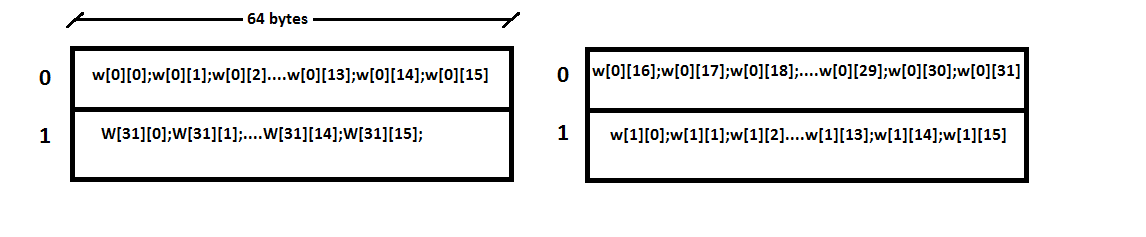
\includegraphics[width=1\textwidth]{Cache.png}
\end{center}
\caption{Situaci\'on ideal del cach\'e.} \label{fig001234}
\end{figure}

La matriz podr\'ia no estar alineada, pero la idea se mantiene. Suponiendo que la ejecuci\'on en ese punto del programa est\'a pasando por la celda [0][1], las direcciones posibles ('NORTH', 'SOUTH', 'WEST', 'EAST') ya est\'an cargadas en cach\'e.

Si este estado se mantuviera, ser\'ia el mejor uso posible para esta cach\'e, que implicar\'ia, a grandes rasgos, un MR de 1/16 (una lectura de una celda del Wator en memoria trae consigo 15 celdas que ser\'an utilizadas pr\'oximamente). Pero entre las llamadas a funciones es necesario acceder a otras direcciones de memoria que remueven un bloque valioso del cach\'e. Si hubiera forma de evitar que algo se cargue en cach\'e desde software, lo hubi\'eramos utilizado
    
% Citas bibliogr\'aficas.
\begin{thebibliography}{99}

\bibitem{HEN00} J. L. Hennessy and D. A. Patterson, ``Computer Architecture. A Quantitative
Approach,'' 3ra Edici\'on, Morgan Kaufmann Publishers, 2000.

\bibitem{HEN01} ``Sharks and fish wage an ecological war on toroidal planet WATOR'', A.K.Dewdney, Scientific American,\\
http://home.cc.gatech.edu/biocs1/uploads/2/wator\_dewdney.pdf.

\bibitem{HEN02} WA-TOR, Wikipedia, http://en.wikipedia.org/wiki/Wa-Tor.

\bibitem{HEN03} GNU profiler, http://sourceware.org/binutils/.

\bibitem{HEN04} Cachegrind, http://valgrind.org/docs/.

\bibitem{HEN05} GCC Options that Control Optimization - http://gcc.gnu.org/onlinedocs/gcc/Optimize-Options.html

\bibitem{HEN06} Steve McConnell, ``Code Complete'' 2nd Edition 2004 - Chapter 26 ``Code-Tunning Techniques''

\end{thebibliography}

\end{document}
